\chapter{Wstęp}

Metrologia optyczna stanowi obecnie jeden z najważniejszych narzędzi pomiarowych w nauce i przemyśle, stale zwiększając swoje znaczenie. Bezdotykowy pomiar temperatury rewolucjonizuje precyzję kontroli procesów technologicznych, badań naukowych i diagnostyki medycznej. Szczególną zaletą tych rozwiązań jest możliwość wykonywania pomiarów w warunkach, które dotychczas stanowiły wyzwanie – w przypadku obiektów szybko się poruszających, materiałów o ekstremalnych temperaturach lub gdy klasyczny kontakt pomiarowy mógłby zakłócić naturalne właściwości badanego obiektu i wprowadzić zaburzenie do pomiaru.

\vspace{12pt}

Zakres niniejszego projektu obejmuje kompleksowe opracowanie optycznego pomiaru temperatury, który łączy optymalne rozwiązania zarówno w obszarze sprzętowym, jak i programowym. Projekt podzielony jest na dwie główne części: część sprzętową i programową. Pod uwagę wzięte zostaną także różnorodne istotne czynniki, które wpływają na sposób wykorzystania zbudowanego urządzenia. Kluczowe dla projektu jest nie tylko samo działanie pirometru, lecz także wpływ środowiska, w którym jest użytkowane, i kwestia racjonalnej minimalizacji kosztów utworzenia w pełni funkcjonalnego systemu pomiarowego.

\vspace{12pt}

Po wstępie i założeniach projektowych następuje szczegółowy opis części sprzętowej oraz programowej systemu. Raport obejmuje proces uruchomienia i kalibracji urządzenia wraz z wynikami pomiarów testowych. Dla użytkowników przygotowano instrukcję obsługi. Całość uzupełniają podsumowanie, dodatki oraz bibliografia.

\chapter{Wprowadzenie}

%\section*{Temperatura}

%\newpage

\textbf{Temperatura} jest fundamentalnym parametrem fizycznym, który charakteryzuje stan energetyczny układu termodynamicznego. Stanowi ona miarę średniej energii kinetycznej cząsteczek materii, objawiającej się poprzez ich chaotyczny ruch i drgania. W praktyce inżynierskiej i życiu codziennym temperatura jest kluczowym parametrem determinującym kierunek przepływu energii cieplnej między ciałami oraz wpływającym na właściwości fizyczne materiałów.

\vspace{12pt}

W układzie SI przyjęto skalę Kelwina (K) jako podstawową jednostkę temperatury, definiując ją poprzez stałą Boltzmanna i energię kinetyczną cząsteczek. Historycznie wykształciły się również inne skale temperatur - skala Celsjusza (°C), powszechnie stosowana w Europie, oraz skala Fahrenheita (°F), popularna głównie w Stanach Zjednoczonych. Każda z tych skal ma swoje charakterystyczne punkty odniesienia, co przedstawiono w tabeli \ref{tab:skale_temperatur}.

\vspace{12pt}

\begin{table}[h]
\centering
\begin{tabular}{|l|c|c|c|}
\hline
\multirow{2}{*}{\textbf{Punkt charakterystyczny}} & \multicolumn{3}{c|}{\textbf{Skala temperatur}} \\
\cline{2-4}
& \textbf{Fahrenheit} & \textbf{Kelvin} & \textbf{Celsjusz} \\
\hline
\multicolumn{4}{|c|}{\textit{Punkty podstawowe}} \\
\hline
Zero bezwzględne & -459,67 & 0 & -273,15 \\
Zero Fahrenheita & 0 & 255,37 & -17,78 \\
\hline
\multicolumn{4}{|c|}{\textit{Punkty charakterystyczne wody}} \\
\hline
Zamarzanie & 32 & 273,15 & 0 \\
Wrzenie & 212 & 373,15 & 100 \\
\hline
\multicolumn{4}{|c|}{\textit{Temperatura biologiczna}} \\
\hline
Średnia temp. ciała człowieka & 98,2 & 309,8 & 36,6 \\
\hline
\end{tabular}
\caption{Porównanie podstawowych skal temperatury}
\label{tab:skale_temperatur}
\end{table}

Szczególne znaczenie w fizyce ma pojęcie zera bezwzględnego (0 K), które stanowi teoretyczną granicę najniższej możliwej temperatury. W tej temperaturze ustaje ruch termiczny cząsteczek, a układ osiąga minimum energii. Jest to stan nieosiągalny w praktyce, choć współczesne laboratoria potrafią zbliżyć się do niego na milionowe części Kelwina.

\vspace{16pt}

Temperatura odgrywa kluczową rolę w procesach wymiany ciepła. Zgodnie z drugą zasadą termodynamiki, energia cieplna przepływa samorzutnie tylko w jednym kierunku - od ciał o wyższej temperaturze do ciał o temperaturze niższej. Proces ten trwa do momentu osiągnięcia równowagi termodynamicznej, czyli wyrównania temperatur wszystkich ciał uczestniczących w wymianie ciepła. Ta fundamentalna zasada ma istotne znaczenie w projektowaniu systemów pomiarowych i kontroli procesów przemysłowych.

\vspace{12pt}

W metrologii optycznej pomiar temperatury opiera się na fundamentalnej własności materii - emisji promieniowania termicznego. Każde ciało o temperaturze wyższej od zera bezwzględnego emituje promieniowanie elektromagnetyczne, którego charakterystyka spektralna i intensywność są ściśle powiązane z jego temperaturą. Współczesne metody pomiaru wykorzystują to zjawisko na kilka sposobów.

%\section{Sposoby pomiaru temperatury}

\vspace{12pt}

\textbf{Podstawowe metody pomiaru temperatury} można sklasyfikować na dwie główne kategorie: stykowe i bezstykowe jak pokazano na rysunku \ref{fig:metody}. Kluczowy jest sposób oddziaływania czujnika z obiektem. Metody stykowe wymagają fizycznego kontaktu czujnika z powierzchnią obiektu, co pozwala na przekazywanie ciepła poprzez przewodzenie. Z kolei metody bezstykowe opierają się na detekcji promieniowania cieplnego emitowanego przez obiekty, które mają temperaturę wyższą niż zero absolutne (0 K). Każdy obiekt emituje to promieniowanie, co umożliwia pomiar bez konieczności bezpośredniego dotyku.

\vspace{12pt}

Technologie bezstykowe, takie jak pirometry podczerwieni czy kamery termowizyjne, zrewolucjonizowały sposób monitorowania temperatury, oferując szybkie, precyzyjne i bezpieczne pomiary nawet na odległość. Są one nieocenione w zastosowaniach przemysłowych, medycznych czy naukowych, gdzie bezpośredni kontakt z obiektem może być trudny, niebezpieczny lub wręcz niemożliwy. Warto jednak pamiętać, że w przypadku ciał stałych i cieczy promieniowanie cieplne pochodzi głównie z warstwy przypowierzchniowej, dlatego kluczowe jest uwzględnienie współczynnika emisyjności materiału, aby uniknąć błędów w interpretacji wyników.

\vspace{12pt}

Co więcej, rozwój technologii bezstykowych wpływa również na minimalizację wpływu na badane obiekty. W przypadku delikatnych materiałów czy żywych organizmów, metody bezstykowe eliminują ryzyko uszkodzenia czy zniekształcenia wyników pomiarów.

\vspace{12pt}

\begin{figure}[h!]
    \centering
    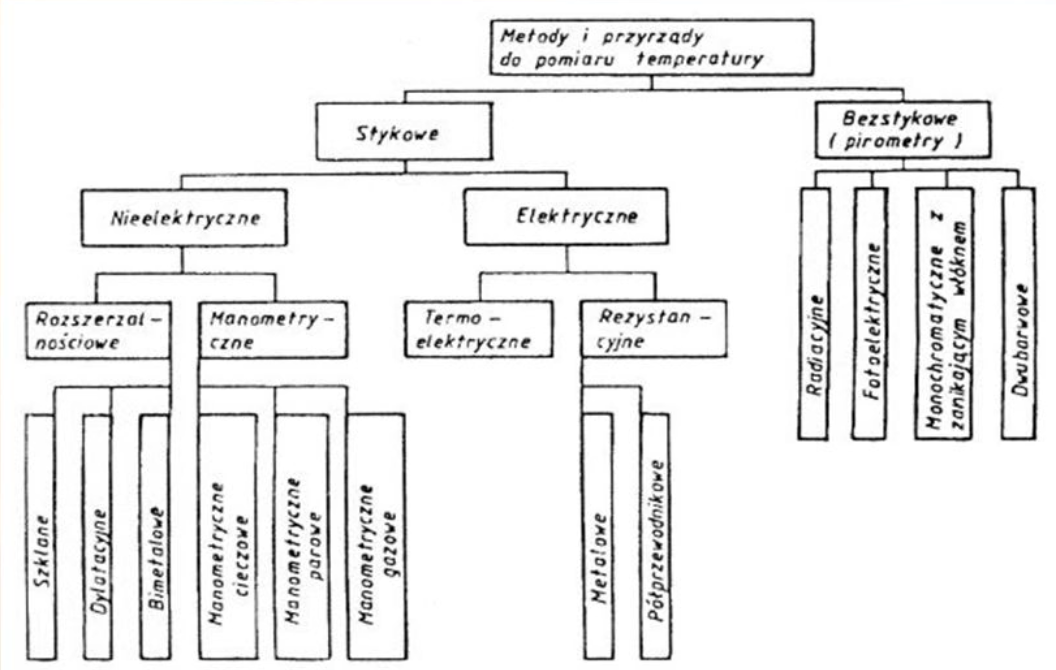
\includegraphics[width=0.75\textwidth]{images/metody.png}
    \caption{Podstawowe metody pomiaru temperatury} \cite{1}
    \label{fig:metody}
\end{figure}

%\vspace{12pt}

Współczesne rozwiązania pomiarowe idą jednak o krok dalej, integrując zaawansowane algorytmy przetwarzania obrazu termicznego oraz techniki sztucznej inteligencji. Dzięki temu możliwe jest nie tylko dokładniejsze monitorowanie temperatury, ale także automatyzacja procesów decyzyjnych. Przykładowo, systemy oparte na AI mogą analizować trendy temperaturowe w czasie rzeczywistym, przewidywać potencjalne awarie w maszynach czy optymalizować zużycie energii w inteligentnych budynkach. To otwiera nowe możliwości w zarządzaniu energią, diagnostyce medycznej czy nawet w badaniach klimatycznych.

\section*{Zasada działania pirometru}

Każdy przedmiot materialny emituje promieniowanie podczerwone (cieplne), niewidoczne dla oczu, ale wyczuwalne np. przy zbliżeniu ręki do gorącego żelazka. Natężenie tego promieniowania jest tym większe, im wyższa jest temperatura przedmiotu. Pirometr mierzy natężenie promieniowania podczerwonego dochodzącego od przedmiotu do jego obiektywu. Zmierzoną wielkość promieniowania przyrząd przelicza na odpowiadającą jej temperaturę przedmiotu i pokazuje wartość tej temperatury na wyświetlaczu.

\section*{Pole widzenia pirometru}

Standardowy przenośny pirometr umożliwia pomiar średniej temperatury powierzchni kołowej o średnicy kilku centymetrów z odległości 1 metra. Wraz ze zwiększaniem się odległości pirometru od mierzonego obiektu, rośnie również średnica obszaru, z którego urządzenie rejestruje promieniowanie podczerwone, co doskonale obrazuje rysunek \ref{fig:pole}.

\begin{figure}[h!]
    \centering
    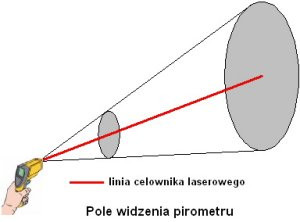
\includegraphics[width=0.7\textwidth]{images/pole.jpg}
    \caption{Zależność pola widzenia od odleglości do mierzonego obiektu} \cite{2}
    \label{fig:pole}
\end{figure}

\vspace{12pt}

Aby ułatwić precyzyjne zlokalizowanie obszaru pomiarowego, pirometry są zazwyczaj wyposażone w celownik laserowy. Promień lasera widoczny jest jako czerwona plamka na powierzchni mierzonego obiektu. Jej położenie wyznacza środek koła, które określa pole widzenia pirometru.

\section*{Pomiary przy użyciu pirometru}

Aby wykonać prawidłowy pomiar, pole widzenia pirometru nie może wychodzić poza przedmiot, którego temperaturę mierzymy. W przeciwnym razie pirometr będzie zbierał promieniowanie podczerwone nie tylko z przedmiotu, ale także z otoczenia ($t_\text{a}$), co spowoduje błędny wynik pomiaru. Na rysunku \ref{fig:pomiar} przedstawiono prawidłowe oraz nieprawidłowe ustawienie pola widzenia pirometru względem powierzchni mierzonego obiektu.

\begin{figure}[h!]
    \centering
    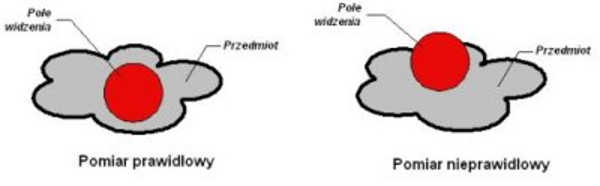
\includegraphics[width=1\textwidth]{images/pomiar.jpg}
    \caption{Prawidłowy i nieprawidłowy pomiar z wykorzystaniem pirometru} \cite{2}
    \label{fig:pomiar}
\end{figure}

\section*{Współczynnik emisyjności powierzchni a dokładność pomiaru}

Materiały mają różną zdolność wysyłania promieniowania podczerwonego ze swojej powierzchni. Właściwość ta zależy od gładkości i barwy powierzchni. Materiały o powierzchniach matowych i ciemnych lepiej emitują promieniowanie podczerwone niż materiały o powierzchniach gładkich i jasnych.

\vspace{12pt}

Współczynnik emisyjności określa się w zakresie od 0 do 1. Przykładowo, współczynnik emisyjności powierzchni cegły wynosi 0.85, a powierzchni polakierowanej czarnym lakierem matowym 0.97. Aluminium ma współczynnik emisyjności 0.07. W celu otrzymania prawidłowego wyniku pomiaru pirometrem należy wartość współczynnika emisyjności danej powierzchni wprowadzić do pamięci wewnętrznej przyrządu.

%\vspace{12pt}

%\section{Ciało doskonale czarne}


%\section{Prawo Wiena} 


%\vspace{12pt}
\section*{Prawa fizyczne i wzory}

\textbf{Prawo Wiena} (\ref{eq:wien}) określa zależność między temperaturą ciała doskonale czarnego a długością fali, przy której emituje ono najwięcej promieniowania. Formuła ta jest wykorzystywana do określania temperatury na podstawie emitowanego promieniowania.

\begin{equation}
    \lambda_{MAX} = \frac{b}{T}
    \label{eq:wien}
\end{equation}

gdzie:
\begin{itemize}
    \item $\lambda_{MAX}$ – długość fali o maksymalnej emisji,
    \item $T$ – temperatura,
    \item $b$ – stała Wiena.
\end{itemize}

\vspace{12pt}

\textbf{Prawo Stefana-Boltzmanna} (\ref{eq:boltz}) mówi, że całkowita energia promieniowania ciała doskonale czarnego jest proporcjonalna do czwartej potęgi jego temperatury

\vspace{12pt}

\begin{equation}
    E = \sigma T^4
    \label{eq:boltz}
\end{equation}

%\vspace{12pt}

% Poniżej przedstawiono zestaw wzorów opisujących wymianę ciepła przez promieniowanie oraz związane z nimi parametry fizyczne:

% \begin{itemize}
%     \item \(\sigma\) – stała Stefana-Boltzmanna, określająca intensywność promieniowania ciała doskonale czarnego,
%     \item \(\epsilon\) – współczynnik emisyjności (od 0 do 1), opisujący zdolność ciała do emitowania promieniowania w stosunku do ciała doskonale czarnego,
%     \item \(S\) – powierzchnia ciała emitującego promieniowanie,
%     \item \(T_{\text{env}}\) – temperatura otoczenia w stopniach Celcjusza (°C),
%     \item \(T_{\text{meas}}\) – zmierzona temperatura obiektu stopniach Celcjusza (°C),
%     \item \(T_{\text{real}}\) – rzeczywista temperatura obiektu stopniach Celcjusza (°C).
% \end{itemize}

% %\section{Wzory}
% 1. Moc promieniowania cieplnego emitowanego przez ciało:
% \[
% P = \sigma \cdot \epsilon \cdot S \cdot \left( T_{\text{env}}^4 - T^4 \right)
% \]

% 2. Równanie równowagi cieplnej opisujące emisję promieniowania:
% \[
% \epsilon \cdot T_{\text{env}}^4 - \epsilon \cdot T_{\text{real}}^4 = T_{\text{env}}^4 - T_{\text{meas}}^4
% \]

\textbf{Ciało doskonale czarne} to teoretyczny obiekt fizyczny, który całkowicie pochłania padające na niego promieniowanie elektromagnetyczne, niezależnie od długości fali. Nie odbija ani nie przepuszcza żadnego promieniowania. W praktyce ciało doskonale czarne jest również idealnym emitentem promieniowania cieplnego, co oznacza, że emituje maksymalną możliwą ilość promieniowania dla danej temperatury. Jego emisyjność wynosi 1.

\vspace{12pt}

\begin{figure}[h!]
    \centering
    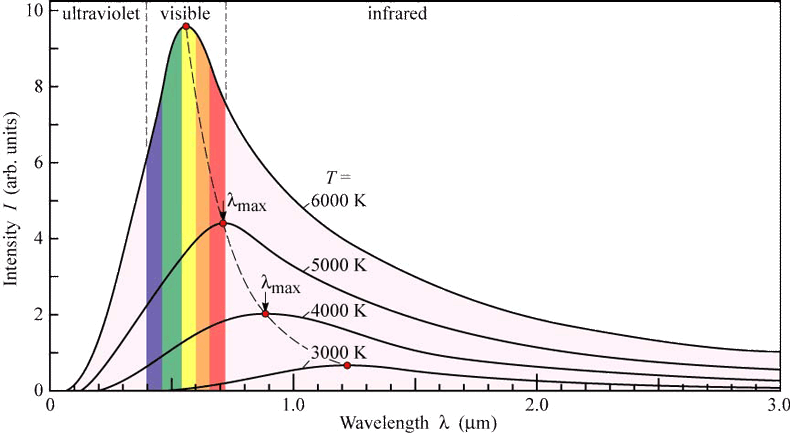
\includegraphics[width=0.9\textwidth]{images/wave.png}
    \caption{Rozkład energii w widmie promieniowania ciała doskonale czarnego w różnych temperaturach} \cite{3}
    \label{fig:pomiar}
\end{figure}

\vspace{12pt}

\textbf{Współczynnik emisyjności} ($\varepsilon$) opisuje, jaką część energii promieniowania emitowanego przez ciało doskonale czarne emituje dane ciało w tej samej temperaturze. Wartość współczynnika emisyjności $\varepsilon$ jest zazwyczaj dostarczana przez producenta.

\vspace{12pt}

Współczynnik emisyjności obliczony na podstawie zmierzonych temperatur:
% \[
% \epsilon = \frac{T_{\text{env}}^4 - T_{\text{meas}}^4}{T_{\text{env}}^4 - T_{\text{real}}^4}
% \]

% \begin{itemize}
%     %\item \(\sigma\) – stała Stefana-Boltzmanna, określająca intensywność promieniowania ciała doskonale czarnego,
%     %\item \(\epsilon\) – współczynnik emisyjności (od 0 do 1), opisujący zdolność ciała do emitowania promieniowania w stosunku do ciała doskonale czarnego,
%     %\item \(S\) – powierzchnia ciała emitującego promieniowanie,
%     \item \(T_{\text{env}}\) – temperatura otoczenia w stopniach Celcjusza (°C),
%     \item \(T_{\text{meas}}\) – zmierzona temperatura obiektu stopniach Celcjusza (°C),
%     \item \(T_{\text{real}}\) – rzeczywista temperatura obiektu stopniach Celcjusza (°C).
% \end{itemize}

\[
\varepsilon = \frac{T_{O_1}^4 - T_{A_1}^4}{T_{O_2}^4 - T_{A_2}^4}
\]

gdzie:
\begin{itemize}
    \item $T_{O_1}$ – zmierzona temperatura obiektu (w kelwinach),
    \item $T_{A_1}$ – zmierzona temperatura otoczenia (w kelwinach),
    \item $T_{O_2}$ – rzeczywista temperatura obiektu (w kelwinach),
    \item $T_{A_2}$ – rzeczywista temperatura otoczenia (w kelwinach).
\end{itemize}

%Na podstawie dwóch różnych temperatur wyznaczono emisyjność badanego obiektu. 

    %Celem niniejszego projektu jest opracowanie i implementacja pirometru – zaawansowanego urządzenia do bezdotykowego pomiaru temperatury wykorzystującego technologię podczerwieni. Projekt został zrealizowany w oparciu o czujnik MLX90614, który zapewnia odpowiednią precyzję i stabilność pomiarów w założonym zakresie temperatur. Sercem systemu jest popularna płytka mikrokontrolerowa, Arduino UNO, która stanowi centrum sterujące całego urządzenia. Płytka Arduino UNO oparta jest na 8-bitowym mikrokontrolerze ATmega328P, który zapewnia różnorodne funkcje, takie jak 14 cyfrowych pinów wejścia/wyjścia czy 6 analogowych wejść. Dzięki swojej prostocie i wszechstronności, Arduino UNO jest często pierwszym wyborem dla wielu, nieco mniej wymagających obliczeniowo projektów \cite{1}. Kod źródłowy projektu został napisany w języku C/C++, z wykorzystaniem open-sourcowych bibliotek ułatwiających programowanie kluczowych komponentów, w tym wyświetlacza LCD opartego na standardzie HD44780. HD44780 to standardowy kontroler wyświetlaczy LCD. Został opracowany przez firmę Hitachi w latach 80. XX wieku i jest powszechnie stosowany w alfanumerycznych wyświetlaczach dot-matrix \cite{2}. W projektach wykorzystujących tę technologię często stosowana jest biblioteka LiquidCrystalI2C, która upraszcza interakcję z wyświetlaczami LCD podłączonymi do mikrokontrolerów takich jak Arduino poprzez interfejs I2C. Dzięki tej bibliotece możliwe jest łatwe sterowanie wyświetlaczem oraz wyświetlanie tekstu i danych w sposób efektywny i intuicyjny. 

    %\vspace{12pt}
    
    %Inicjalizacja omawianego wyświetlacza LCD z wykorzystaniem biblioteki LiquidCrystalI2C zajmuje zaledwie kilka linijek kodu źródłowego:

    %\begin{lstlisting}[style=mystyle]
    %    #include <LiquidCrystal_I2C.h>
    %    LiquidCrystal_I2C lcd(0x27, 16, 2); // Adres I2C, liczba kolumn, liczba wierszy
    %    \end{lstlisting}
    
    %\section{Zakres projektu}
